%%
%% Automatically generated file from DocOnce source
%% (https://github.com/hplgit/doconce/)
%%
%%


%-------------------- begin preamble ----------------------

\documentclass[%
oneside,                 % oneside: electronic viewing, twoside: printing
final,                   % draft: marks overfull hboxes, figures with paths
10pt]{article}

\listfiles               %  print all files needed to compile this document

\usepackage{relsize,makeidx,color,setspace,amsmath,amsfonts,amssymb}
\usepackage[table]{xcolor}
\usepackage{bm,ltablex,microtype}

\usepackage[pdftex]{graphicx}

\usepackage{fancyvrb} % packages needed for verbatim environments

\usepackage[T1]{fontenc}
%\usepackage[latin1]{inputenc}
\usepackage{ucs}
\usepackage[utf8x]{inputenc}
\usepackage{comment}
\usepackage{listings}
\usepackage{lmodern}         % Latin Modern fonts derived from Computer Modern

% Hyperlinks in PDF:
\definecolor{linkcolor}{rgb}{0,0,0.4}
\usepackage{hyperref}
\hypersetup{
    breaklinks=true,
    colorlinks=true,
    linkcolor=linkcolor,
    urlcolor=linkcolor,
    citecolor=black,
    filecolor=black,
    %filecolor=blue,
    pdfmenubar=true,
    pdftoolbar=true,
    bookmarksdepth=3   % Uncomment (and tweak) for PDF bookmarks with more levels than the TOC
    }
%\hyperbaseurl{}   % hyperlinks are relative to this root

\setcounter{tocdepth}{2}  % levels in table of contents

% --- fancyhdr package for fancy headers ---
\usepackage{fancyhdr}
\fancyhf{} % sets both header and footer to nothing
\renewcommand{\headrulewidth}{0pt}
\fancyfoot[LE,RO]{\thepage}
% Ensure copyright on titlepage (article style) and chapter pages (book style)
\fancypagestyle{plain}{
  \fancyhf{}
  \fancyfoot[C]{{\footnotesize \copyright\ 1999-2018, "Computational Physics I FYS3150/FYS4150":"http://www.uio.no/studier/emner/matnat/fys/FYS3150/index-eng.html". Released under CC Attribution-NonCommercial 4.0 license}}
%  \renewcommand{\footrulewidth}{0mm}
  \renewcommand{\headrulewidth}{0mm}
}
% Ensure copyright on titlepages with \thispagestyle{empty}
\fancypagestyle{empty}{
  \fancyhf{}
  \renewcommand{\footrulewidth}{0mm}
  \renewcommand{\headrulewidth}{0mm}
}

\pagestyle{fancy}


% prevent orhpans and widows
\clubpenalty = 10000
\widowpenalty = 10000

% --- end of standard preamble for documents ---


% insert custom LaTeX commands...

\raggedbottom
\makeindex
\usepackage[totoc]{idxlayout}   % for index in the toc
\usepackage[nottoc]{tocbibind}  % for references/bibliography in the toc

%-------------------- end preamble ----------------------

\usepackage{parskip}
\usepackage{verbatim}

\begin{document}
%\setlength{\parindent}{0pt}


% matching end for #ifdef PREAMBLE

\newcommand{\exercisesection}[1]{\subsection*{#1}}


% ------------------- main content ----------------------



% ----------------- title -------------------------

\thispagestyle{empty}

\begin{center}
{\LARGE\bf
\begin{spacing}{1.25}
FYS3150 - Project 1
\end{spacing}
}
\end{center}



\begin{center}
\centerline{{\small Ingvild Bergsbak, Erlend Ousdal and Oliver Hebnes}}
\end{center}



\begin{center}
September 10, 2018
\end{center}
% --- end date ---

\vspace{1cm}

\newpage{}


\section{Abstract}

We study the one-dimensional Poissons equation with Dirichlet boundary conditions by rewriting it as a set of linear equations.
The result is verified versus the exact solution. We find that increasing the number of grid points
will result in a smaller error.

Time --> general tridiagonal vs LU ?  (flops?)

\section{Introduction}

This project is our first encounter with the programming language C++ and the subject computational physics.
We have tried writing and understanding code in both Python and C++ and we are going to compare the two programming languages against each other, with
the use of dynamical memory allocation to the usage of some programs in the library package of the course.

The learning curve has been very steep, but it is very motivating getting understandable results.


\section{Theoretical Models and Technicalities}

The purpose of this project is to solve the Poisson equation numerically. We have the equation
\begin{equation*}
-u''(x) = f(x), \hspace{0.5cm} x\in(0,1), \hspace{0.5cm} u(0) = u(1) = 0.
\end{equation*}
and we approximate the second derivative of $u$ by
\begin{equation*}
-u''(x_i)\approx -\frac{v_{i+1}+v_{i-1}-2v_i}{h^2} = f_i  \hspace{0.5cm} \mathrm{for} \hspace{0.1cm} i=1,\dots, n,
\end{equation*}
where $f_i=f(x_i)$.



We define the discretized approximation  to $u$ as $v_i$  with
grid points $x_i=ih$ where $h$ is defined as $h=1/(n+1)$ and $x$ is in the interval from $x_0=0$ to $x_{n+1}=1$.

We have the boundary conditions $v_0 = v_{n+1} = 0$.


Rewriting the approximation gives

\begin{equation*}
-v_{i+1}+2v_{i}-v_{i-1} = h^2f_i=\tilde{b}_i
\end{equation*}


Solving for a slection of $i$ values reveals a pattern\\
\begin{align*}
  i &=1: -v_{2}+2v_{1}-v_0 = -v_{2}+2v_1=\tilde{b}_1\\
  i &=2: -v_{3}+2v_{2}-v_1 = \tilde{b}_2\\
  i &=3: -v_{4}+2v_{3}-v_2 = \tilde{b}_3\\
  \vdots\\
  i &=n: -v_{n+1}+2v_n-v_{n-1} = -v_{n-1}+2v_{n}=\tilde{b}_n\\
\end{align*}

and the equation, $v_{i+1}+v_{i-1}-2v_i =\tilde{b}_i$, can be written as
$$\mathbf{Av}=\mathbf{\tilde{b}} $$\\

where

\begin{equation*}
\mathbf{A}=\begin{bmatrix}
2 & -1 & 0 & \cdots & 0\\
-1 & 2 & -1 & & \\
0 & -1 & 2 & & \vdots \\
\vdots & & & \ddots &-1\\
0 & \cdots & 0 & -1 & 2
\end{bmatrix},
\mathbf{v}=
\begin{bmatrix}
v_1\\
v_2\\
v_3\\
\vdots\\
v_n
\end{bmatrix},
\mathbf{\tilde{b}}=\begin{bmatrix}
\tilde{b}_1\\
\tilde{b}_2\\
\tilde{b}_3\\
\vdots\\
\tilde{b}_n\\
\end{bmatrix}
\end{equation*}

and $\mathbf{A}$ is a $n\times n$ matrix.

\vskip0.7cm
The function $f$ is defined as
$$f(x)=100e^{-10x}$$

Checking the exact solution $u(x)=1-(1-e^{-10})x-e^{-10x}$ by inserting $f$ and $u$ into the Poisson equation.

$$-u''(x)=f(x)$$

\begin{equation*}
\begin{split}
\frac{d^2}{dx^2}u&=\frac{d^2}{dx^2}(1-x+e^{-10}x-e^{-10x})\\
&=\frac{d}{dx}(1+e^{-10}+10e^{-10x})\\
&=-100e^{-10x} = -f(x)
\end{split}
\end{equation*}

Can see that $-u''(x)$ is equal to $f(x)$, and the Poisson equation is satisfied.

\vskip1cm




Gaussian elimination is a very useful method for solving a large set of equations, which can be represented by the form $\mathbf{Av}=\mathbf{b}$. In our case the matrix, $\mathbf{A}$, is a tridigonal matrix, which allows us to simplify the method further.

%---------maybe we dont need the explanation of the tridiag matrix
A tridiagonal matrix is a $n\times n$ matrix with numbers along the diagonal and at the positions directly above and below the diagonal and zeroes on all other positions. To visualize it, the form is shown below.
\begin{equation*}
\mathbf{A}=\begin{bmatrix}
b_1 & c_1 & 0 & \cdots & 0\\
a_1 & b_2 & c_2 & & \\
0 & a_2 & b_3 & & \vdots \\
\vdots & & & \ddots & c_{n-1}\\
0 & \cdots & 0 & a_{n-1} & b_n
\end{bmatrix}
\end{equation*}



First, we use forward substitution, which uses Gaussian elimination to get the matrix on the echolon form, which in this case means $a_i=0$. The Gaussian elimination requires the elements along the diagonal in $\mathbf{A}$ and $\mathbf{\tilde{b}}$ to be updated. The algorithm for this process is given by

\begin{equation*}
\begin{split}
b_i'&=b_i-\frac{a_{i-1}c_{i-1}}{b_{i-1}'}\\
\tilde{b}_i'&=\tilde{b}_i-\frac{a_{i-1}d_{i-1}}{b_{i-1}'}
\end{split}
\end{equation*}

where $b_i'$ and $\tilde{b}_i'$ represent the updated values of $\mathbf{b}$ and $\mathbf{\tilde{b}}$ and $i=1, 2, ..., n$.

Now we are able to solve the equation by backward substitution. This algorithm is given by

\begin{equation*}
\begin{split}
v_n&=b_n'\\
v_i&=\frac{1}{b_i'}(\tilde{b_i}'-c_iv_{i+1})\\
\end{split}
\end{equation*}

where $i=n-1, n-2, ..., 1$.

The theory behind the algorithms for forward and backward substitution are thoroughly described in the lecture notes (Hjort-Jensen, M., 2015 $Computational$ $Physics$), and therefore we will not repeat it in this report.

First we wanted to write a script that would solve the equation $\mathbf{Av}=\mathbf{b}$ for general numbers,
$a_i, b_i$ and $c_i$. We used the matrix $\mathbf A$, but we wrote the algorithm as if the matrix contained random numbers along the diagonals, as shown below. 
\begin{lstlisting}
s=a[i-1]/b[i-1]
b[i] = b[i]-s*c[i-1];
b_tilde[i]=b_tilde[i]-s*b_tilde[i-1]
\end{lstlisting}

Later we wanted to specialize our code to the Poisson equation by implementing the additional information we knew about the matrix, which is the fact that $a_i=c_i=-1$ and $b_i=2$ for $i=1, 2, ..., n$. The difference in the algorithm is one line in the forward substitution algorithm, where we define the updated $b_i$ values, which is changed to

\begin{lstlisting}
b[i] = b[0]-1./b[i-1];
\end{lstlisting}
for the special case because we know that $a_i=c_i=-1$ for all $i=1, 2, ..., n$.






\newpage{}
\section{Results and Discussion}
From figure 1-3 it is pretty obvious that increasing the number of grid points makes the error decrease.
The number of flops from the general algorithm is $5N$ from the forward substitution and $3N+1$ flops
from the backward substitution, making it a total of $8N+1$ flops. 

\begin{figure}
  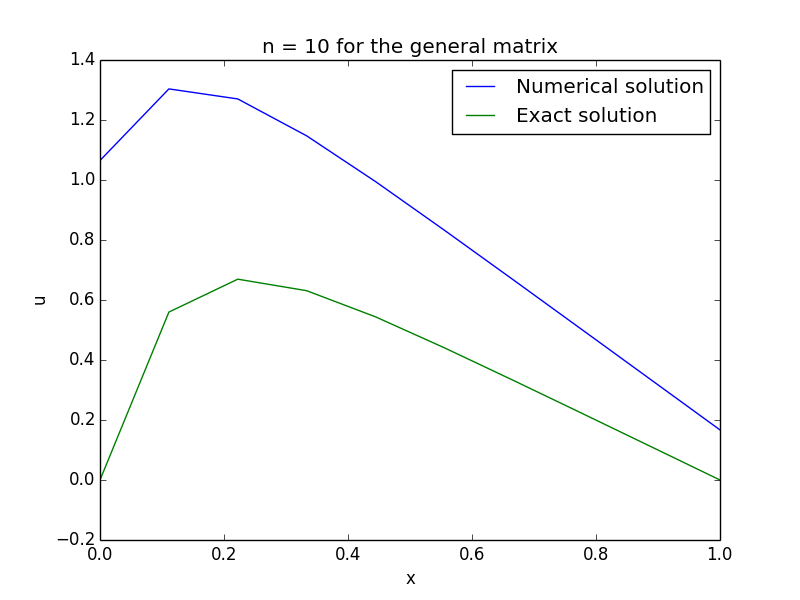
\includegraphics[scale=0.5]{figur1b_10.png}
  \centering
  \caption{Matrix with the size of 10 x 10 compared to the closed-form solution.}
  \label{1b_10}
\end{figure}
\begin{figure}
  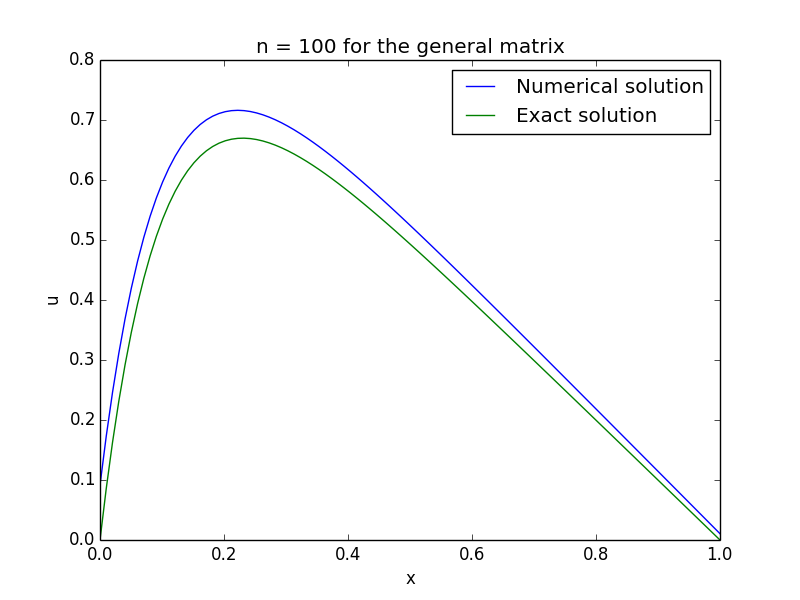
\includegraphics[scale=0.5]{figur1b_100.png}
  \caption{Matrix with the size of 100 x 100 compared to the closed-form solution.}
  \label{1b_100}
\end{figure}

\begin{figure}
  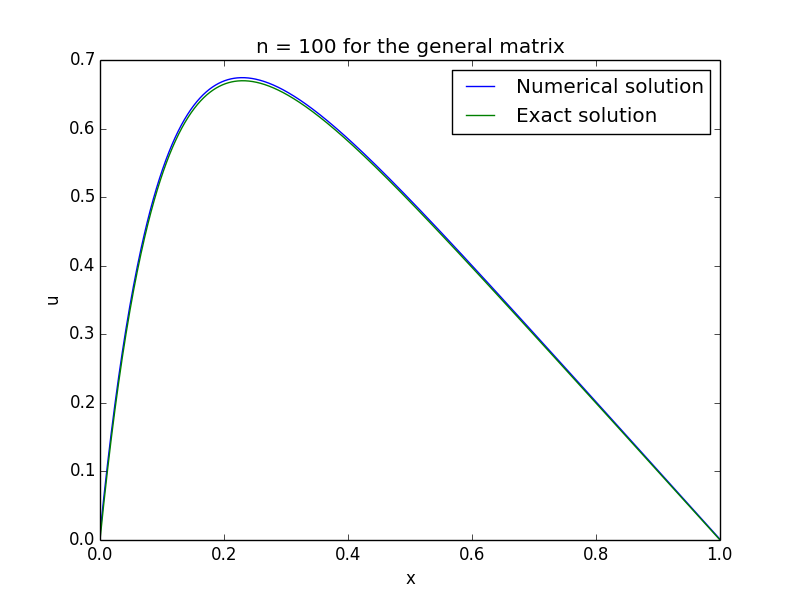
\includegraphics[scale=0.5]{figur1b_1000.png}
  \caption{Matrix with the size of 1000 x 1000 compared to the closed-form solution.}
  \label{1b_1000}
\end{figure}
\newpage{}
\section{Conclusion and Perspective}

\section{Appendix}

\section{Bibliography}

- Hjort-Jensen, M., 2015 $Computational$ $physics$, accesible at course github repository. 551 pages.































\begin{comment}
\paragraph{Project 1 b):}
We can rewrite our matrix $\mathbf{A}$ in terms of one-dimensional vectors $a,b,c$
of length $1:n$.
Our linear equation reads

\[
    \mathbf{A} = \begin{bmatrix}
                           b_1& c_1 & 0 &\dots   & \dots &\dots \\
                           a_1 & b_2 & c_2 &\dots &\dots &\dots \\
                           & a_2 & b_3 & c_3 & \dots & \dots \\
                           & \dots   & \dots &\dots   &\dots & \dots \\
                           &   &  &a_{n-2}  &b_{n-1}& c_{n-1} \\
                           &    &  &   &a_{n-1} & b_n \\
                      \end{bmatrix}\begin{bmatrix}
                           v_1\\
                           v_2\\
                           \dots \\
                          \dots  \\
                          \dots \\
                           v_n\\
                      \end{bmatrix}
  =\begin{bmatrix}
                           \tilde{b}_1\\
                           \tilde{b}_2\\
                           \dots \\
                           \dots \\
                          \dots \\
                           \tilde{b}_n\\
                      \end{bmatrix}.
\]




Note well that we do not include the endpoints since the boundary
conditions are used resulting in a fixed value for $v_i$.  A
tridiagonal matrix is a special form of banded matrix where all the
elements are zero except for those on and immediately above and below
the leading diagonal.  Develop a general algorithm first which does
not assume that we have a matrix with the same elements along the
diagonal and the non-diagonal elements.  The algorithm for solving
this set of equations is rather simple and requires two steps only, a
decomposition and forward substitution and finally a backward
substitution.

Before we proceed with the solution of the differential equation, you should now plan the organization of your data flow. Here you will find it convenient to define vectors that will contain the matrix elements, the solution to the problem and the function $f(x)$ when discretized. You should also plan on to read input data, whether you do this from the command line or from a selected file. We recommend strongly that you use dynamical memory allocation.
An example of a C++ program which reads from the command line various input parameters can \href{{https://github.com/CompPhysics/ComputationalPhysicsMSU/blob/master/doc/Projects/2018/Project1/CodeExamples/TridiagonalSimple.cpp}}{be found here}

Your first task is to set up the general algorithm (assuming different
values for the matrix elements) for solving this set of linear
equations.  Find also the precise number of floating point operations
needed to solve the above equations. For the general algorithm you
need to specify the values of the array elements $a$, $b$ and $c$ by
inserting their explicit values.


Then you should code the above algorithm and solve the problem for matrices of the size
$10\times 10$, $100\times 100$ and $1000\times 1000$.  That means that you select $n=10$, $n=100$ and
$n=1000$ grid points.

Compare your results (make plots) with the closed-form solution for the different number of grid points  in the
interval $x\in(0,1)$.  The different number of grid points corresponds to different step lengths $h$.


\paragraph{Project 1 c):}
Use thereafter the fact that the matrix has identical matrix elements along the diagonal and identical (but different) values for the non-diagonal elements. Specialize your algorithm to the special case and find the number of floating point operations
for this specific tri-diagonal matrix. Compare the CPU time with the general algorithm from the previous point for matrices up to  $n=10^6$ grid points.

\paragraph{Project 1 d):}
Compute the relative error  in the data set $i=1,\dots, n$,by setting up

\[
   \epsilon_i=log_{10}\left(\left|\frac{v_i-u_i}
                 {u_i}\right|\right),
\]
as function of $log_{10}(h)$ for the function values $u_i$ and $v_i$.
For each step length extract the max value of the relative error.
Try to increase $n$ to $n=10^7$.  Make a table of the results and
comment your results. You can use either the algorithm from b) or c).

\paragraph{Project 1 e):}
Compare your results with those from the LU decomposition codes for the matrix of sizes $10\times 10$, $100\times 100$ and
$1000\times 1000$. Here you should use the library functions provided  on the webpage of the course. Alternatively, if you use armadillo as a library, you can use the similar function for LU decomposition.  The armadillo function for the LU decomposition is called $LU$ while the function for solving linear sets of equations is called $solve$.
Use for example the unix function \emph{time} when you run your codes
and compare the time usage between LU decomposition and  your
tridiagonal solver.   Alternatively, you can use the functions in C++, Fortran or Python that measure the time used.

Make a table of the results and comment the differences
in execution time
How many floating point operations does the LU decomposition use to solve the set of linear equations?
Can you run the standard LU decomposition
for a matrix of the size $10^5\times 10^5$?
Comment your results.


To compute the elapsed time in c++ you can use the following statements
\end{comment}

\begin{comment}
...
#include "time.h"   //  you have to include the time.h header
int main()
{
    // declarations of variables
    ...
    clock_t start, finish;  //  declare start and final time
    start = clock();
    // your code is here, do something and then get final time
    finish = clock();
    ( (finish - start)/CLOCKS_PER_SEC );
...

Similarly, in Fortran, this simple example shows how to compute the elapsed time.

PROGRAM time
 REAL :: etime          ! Declare the type of etime()
 REAL :: elapsed(2)     ! For receiving user and system time
 REAL :: total          ! For receiving total time
 INTEGER :: i, j

 WRITE(*,*) 'Start'

 DO i = 1, 5000000
      j = j + 1
 ENDDO

 total = ETIME(elapsed)
 WRITE(*,*) 'End: total=', total, ' user=', elapsed(1), &
              ' system=', elapsed(2)

END PROGRAM time

\end{comment}



\begin{comment}

\subsection*{Introduction to numerical projects}

Here follows a brief recipe and recommendation on how to write a report for each
project.

\begin{itemize}
  \item Give a short description of the nature of the problem and the eventual  numerical methods you have used.

  \item Describe the algorithm you have used and/or developed. Here you may find it convenient to use pseudocoding. In many cases you can describe the algorithm in the program itself.

  \item Include the source code of your program. Comment your program properly.

  \item If possible, try to find analytic solutions, or known limits in order to test your program when developing the code.

  \item Include your results either in figure form or in a table. Remember to        label your results. All tables and figures should have relevant captions        and labels on the axes.

  \item Try to evaluate the reliabilty and numerical stability/precision of your results. If possible, include a qualitative and/or quantitative discussion of the numerical stability, eventual loss of precision etc.

  \item Try to give an interpretation of you results in your answers to  the problems.

  \item Critique: if possible include your comments and reflections about the  exercise, whether you felt you learnt something, ideas for improvements and  other thoughts you've made when solving the exercise. We wish to keep this course at the interactive level and your comments can help us improve it.

  \item Try to establish a practice where you log your work at the  computerlab. You may find such a logbook very handy at later stages in your work, especially when you don't properly remember  what a previous test version  of your program did. Here you could also record  the time spent on solving the exercise, various algorithms you may have tested or other topics which you feel worthy of mentioning.
\end{itemize}

\noindent
\subsection*{Format for electronic delivery of report and programs}

The preferred format for the report is a PDF file. You can also use DOC or postscript formats or as an ipython notebook file.  As programming language we prefer that you choose between C/C++, Fortran2008 or Python. The following prescription should be followed when preparing the report:

\begin{itemize}
  \item Use Devilry to hand in your projects, log in  at  \href{{http://devilry.ifi.uio.no}}{\nolinkurl{http://devilry.ifi.uio.no}} with your normal UiO username and password and choose either 'fys3150' or 'fys4150'. There you can load up the files within the deadline.

  \item Upload \textbf{only} the report file!  For the source code file(s) you have developed please provide us with your link to your github domain.  The report file should include all of your discussions and a list of the codes you have developed.  Do not include library files which are available at the course homepage, unless you have made specific changes to them.

  \item In your git repository, please include a folder which contains selected results. These can be in the form of output from your code for a selected set of runs and input parameters.

  \item In this and all later projects, you should include tests (for example unit tests) of your code(s).

  \item Comments  from us on your projects, approval or not, corrections to be made  etc can be found under your Devilry domain and are only visible to you and the teachers of the course.
\end{itemize}

\noindent
Finally,
we encourage you to work two and two together. Optimal working groups consist of
2-3 students. You can then hand in a common report.

\end{comment}










% ------------------- end of main content ---------------

\end{document}





\begin{equation*}

\end{equation*}
